\chapter{自然语言处理}

\section*{Introduction}
	本章节主要介绍一些文本方面相关的知识。
	

\section{如何表示词}
	\subsection*{Introduction}
	本节主要介绍如何使用词向量的形式去表达一个模型,本章节大部分内容来自知乎专栏以及cs224d课程。
	
	\subsection{one-hot}
	首先,可以将每个词表示成one-hot vector,就是只有在对应位置的向量的值为1,其余位置为0,如下图所示:
	

	\begin{figure}[htbp]
	\centering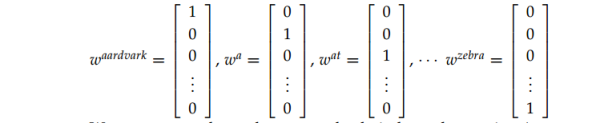
\includegraphics[width=6in]{img/6-1.png}
	\caption{one-hot}\label{fig:6-1}
	\end{figure}
	
	但是这种表示方法有几种缺点,一种是如果词表太长的话,我们可能没有那么多的内存去存储这么多的词向量,另外一种是,每个word之间都是独立的,我们没有办法从中找到他们之间的关系。
	
	\begin{equation}
	(w^{hotel})^{T}(w^{motel}) = (w^{hotel})^{T}(w^{cat})=0
	\end{equation}
	
	虽然两个向量之间的点乘可以表示word之间的关系,但是由于在one-hot中,任意两个向量都是正交的,因此他们之间的点乘结果都是0,所以不能通过这种方式来表达向量之间的相似程度。因此我们需要通过某种方式,将这个高维空间压缩到一个低维的空间中去。	
	
	比如,我们可以通过一个词周围的词来表达这个词的信息。比如如下的例子。可以用banking周围的词来代表banking这个词,这样在大规模的预料中,这样的统计就变得比较重要了。
	
	\begin{figure}[htbp]
	\centering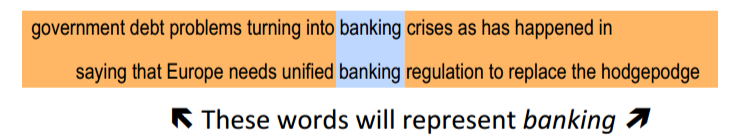
\includegraphics[width=6in]{img/6-2.png}
	\caption{词的表示形式}\label{fig:6-2}
	\end{figure}
	
	这样,我们就可以将之前的one-hot形式的稀疏矩阵变成一个稠密的矩阵了,但是这里的一个词的词向量是从计算机的角度来理解的,没有什么感知上的意义。这样,我们的问题就比较明确了,即找到一个model来刻画一个词和它的上下文之间的概率(即将one-hot变成稠密的矩阵),概率越大说明学习的越好。如果取负值,那么这就是我们的loss function 了。
	
	
	\subsection{skip-gram}
	
	skip-gram是word2vec的其中一种方法,主要的目的是找到一个词和它的上下文之间的关联。word2vec主要有两种模型,两种训练的方法。
	
	skip-gram是一种根据当前的word预测contex的算法。
	
	我们使用如下所示的图来表示skip-gram,加入中心词banking的位置为t,那么我们分别根据第t个词来预测第t-m,...t-1,t+1,...,t+m个词的概率。其中除了第t个词的其他的词叫做output context words。每次计算的时候,取一个词作为中心词
	
	\begin{figure}[htbp]
	\centering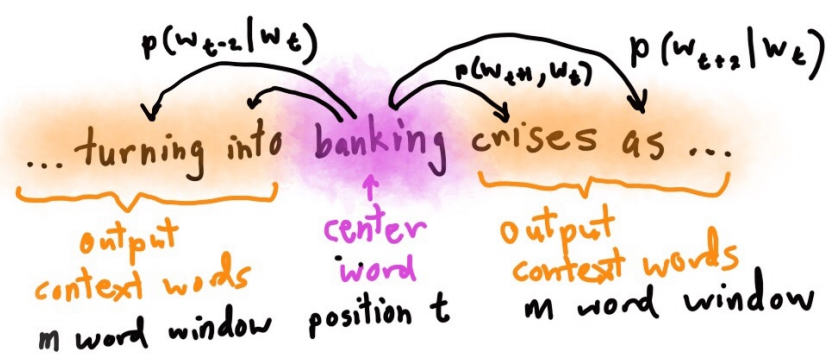
\includegraphics[width=6in]{img/6-3.png}
	\caption{skip-gram}\label{fig:6-3}
	\end{figure}
	
	这样我们就可以获得skip-gram的计算公式了,即分别计算已知第t个词,预测前后m个词的概率,然后最大化概率的成绩即可,对于第二个连乘来说计算的是这一个中心词的所有上下文词的概率,第一个连乘表示的是每次取一个词作为中心词,遍历所有的词。加入负号之后我们即可以直接作为loss function 来使用了。公式如下:
	
	\begin{equation}
		L(\theta) = \prod_{t=1}^{T} \prod_{-m \leq j \leq m} p(w_{t+j}|w_t;\theta)
	\end{equation}
	
	\begin{equation}
		J(\theta) = -\frac{1}{T} \sum_{t=1}^{T} \sum_{-m \leq j \leq m} \log p(w_{t+j}|w_t)
	\end{equation}
	
	通常我们是使用交叉熵来作为损失函数,但是这里的向量使用的是one-hot的形式,计算结果时只有trueclass的位置有值,这样显得不太妥当。
	
	这样我们已经获得了损失函数,下面我们需要做的就仅仅是求出这样一个概率就可以了。概率可以使用如下的公式来求解。同样首先我们需要定义一些表达式:c表示中心词的下标;$v_c$表示第c个中心词的词向量,$u_o$表示第o个outside词的词向量。这样我们就可以表示已知第c个词求第o个词的概率:(这里我们用的是点积,即每个向量对应位置的元素相乘。点乘的意义是两个向量越是接近,点乘的结果越大)
	
	\begin{equation}
	p(o|c) = \frac{exp(u_0^T v_c)}{\sum_{w=1}^v exp(u_w^T v_c)}
	\end{equation}
	
	\begin{figure}[htbp]
	\centering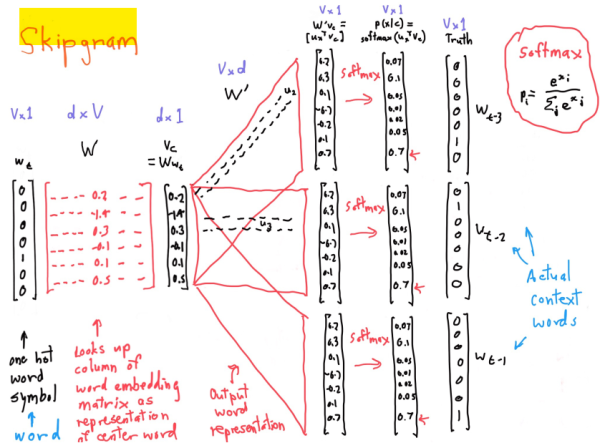
\includegraphics[width=6in]{img/6-4.png}
	\caption{skip-gram}\label{fig:6-4}
	\end{figure}
		
	
	
	
	
	
	\subsection{CBOW}
	CBOW根据surrounding context 来预测center word,对于每一个词,需要学习两个vector,v(input vector):when the word is in the context;u(output):when the word is in the center.
	
	首先我们需要定义一些标准的变量表示方法:
	
	\begin{itemize}
		\item \emph{V} 表示input word matrix
		\item \emph{U} 表示output word matrix;
		\item \ $\omega _i$:表示此表V中的第i个单词
		\item $\nu_i$:表示输入词矩阵中的第i列,是第i个词的input vector
		\item $\mu_i$:表示输出矩阵的第i列,表示第i个词output vector
	
    \end{itemize}	
    
    CBOW的工作流程如下所示:
    \begin{enumerate}
    	\item 首先我们需要产生每一个词的词向量(用one-hot)来表示:$m:(x^{c-m},...,x^{c-1},x^{c},x^{c+1},...,x^{c+m} \in R^{|V|})$,即将contex中的每一个单词都表示成one-hot编码的形式
    	\item 
	\end{enumerate}
	
	
	
	
	
	
	
	
	
	
	
	
	
	
	
	
	
	
	
	
	
	
	
	
	
	
	
	
	    	
	
	